\chapter{Number Theory}
\chapterepigraph{Number theory problems in a prelim are rarely deep --- they
are about knowing five tools cold (Euclid, fast power, Fermat, the sieve and
floor-division blocks) and never overflowing a 64-bit integer.}

\section{Theory and Must-Know Patterns}
\label{sec:nt-theory}

\subsection*{GCD and LCM}

\begin{itemize}
  \item \textbf{Euclid:} $\gcd(a,b)=\gcd(b,a\bmod b)$, $\gcd(a,0)=a$. It takes
        $O(\log\min(a,b))$ steps --- the worst case is consecutive Fibonacci
        numbers.
  \item $\operatorname{lcm}(a,b)=a/\gcd(a,b)\cdot b$ (divide first to avoid
        overflow). C++17 has \texttt{std::gcd} and \texttt{std::lcm} in
        \texttt{<numeric>}.
  \item $\gcd$ is associative, $\gcd(0,x)=x$, so prefix/suffix gcd arrays
        answer ``gcd of everything except $a_i$'' in $O(1)$.
  \item $\gcd(a_\ell,\dots,a_r)=\gcd$ of all adjacent pair gcds in the range.
\end{itemize}

\subsection*{Modular arithmetic}

Work modulo $p=10^9+7$ (prime). Addition, subtraction and multiplication
commute with $\bmod$; keep every intermediate below $p$ and multiply in
\texttt{long long} (or \texttt{\_\_int128} for 64-bit moduli).

\begin{itemize}
  \item \textbf{Fast power:} $a^e$ in $O(\log e)$ by squaring:
        $a^e=(a^{\lfloor e/2\rfloor})^2\cdot a^{e\bmod2}$.
  \item \textbf{Fermat's little theorem:} for prime $p\nmid a$,
        $a^{p-1}\equiv1$, so $a^{-1}\equiv a^{p-2}$ and exponents can be
        reduced modulo $p-1$: $a^e\equiv a^{e\bmod(p-1)}$.
  \item Division by $d$ = multiplication by $d^{p-2}$ (only if $p\nmid d$).
\end{itemize}

\subsection*{Primes and divisors}

\begin{itemize}
  \item \textbf{Sieve of Eratosthenes} up to $V$: $O(V\log\log V)$.
        A ``divisor sieve'' (add $d$ to every multiple) is $O(V\log V)$
        because $\sum_{d\le V}V/d\approx V\ln V$.
  \item For $n=\prod p_i^{k_i}$:
        \[
          \tau(n)=\prod(k_i+1),\qquad
          \sigma(n)=\prod\frac{p_i^{k_i+1}-1}{p_i-1},\qquad
          \prod_{d\mid n}d=n^{\tau(n)/2}.
        \]
  \item Trial division up to $\sqrt n$ factorises $n\le10^{12}$ with
        $10^6$ steps; \textbf{Miller--Rabin} with bases
        $2,3,5,\dots,37$ is exact for all 64-bit integers.
\end{itemize}

\subsection*{Counting tricks}

\begin{itemize}
  \item \textbf{Floor blocks:} $\lfloor n/d\rfloor$ takes at most
        $2\sqrt n$ distinct values; for a block starting at $\ell$ with value
        $q=\lfloor n/\ell\rfloor$ the block ends at $r=\lfloor n/q\rfloor$.
  \item \textbf{Inclusion--exclusion:} the count of $x\le n$ divisible by at
        least one of $a_1,\dots,a_k$ is
        \[
          \sum_{\emptyset\ne S\subseteq\{1..k\}}(-1)^{|S|+1}
          \left\lfloor\frac{n}{\operatorname{lcm}(a_i: i\in S)}\right\rfloor .
        \]
  \item \textbf{Counting multiples:} ``is there a pair with gcd $\ge d$?''
        --- count the multiples of $d$ with a frequency array:
        $\sum_d V/d=O(V\log V)$.
\end{itemize}

\begin{center}
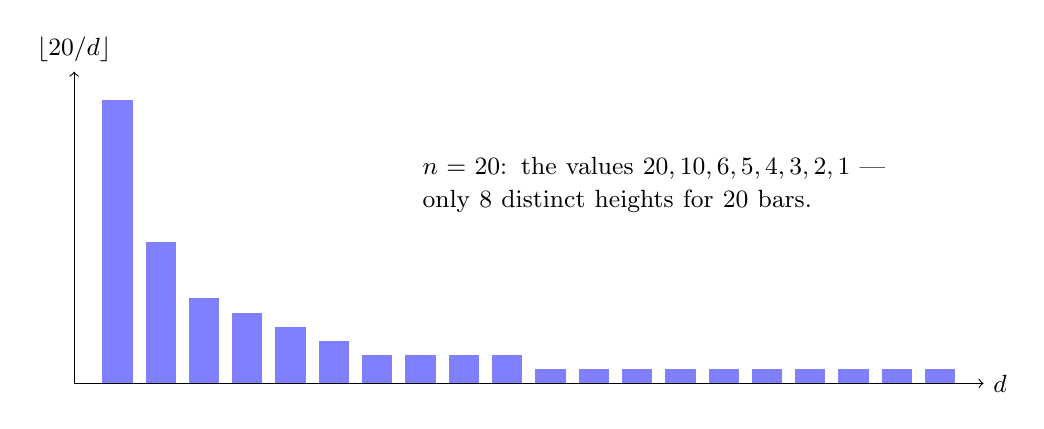
\begin{tikzpicture}[x=0.55cm,y=0.18cm]
  \draw[->] (0,0) -- (21,0) node[right] {\small $d$};
  \draw[->] (0,0) -- (0,22) node[above] {\small $\lfloor 20/d\rfloor$};
  \foreach \d in {1,...,20} {
     \pgfmathtruncatemacro{\q}{20/\d}
     \fill[blue!50] (\d-0.35,0) rectangle (\d+0.35,\q);
  }
  \node[text width=6cm,align=left] at (13.5,14) {\small $n=20$: the values
  $20,10,6,5,4,3,2,1$ --- only $8$ distinct heights for $20$ bars.};
\end{tikzpicture}
\end{center}

\begin{takeawaybox}[Number Theory Checklist]
\begin{enumerate}
  \item Every product of two values below $10^9$ goes in \texttt{long long};
        every product of two values below $10^{18}$ goes in
        \texttt{\_\_int128}.
  \item After subtraction modulo $p$ add $p$ before taking $\bmod$.
  \item Exponents are reduced modulo $p-1$, \emph{not} $p$; watch the base
        $0$.
  \item Special-case $n=1$, $0^0$, and ``no answer'' outputs.
\end{enumerate}
\end{takeawaybox}

\newpage

\section{Calculate GCD}
\label{sec:n-gcd}
\problemlink{https://atcoder.jp/contests/math-and-algorithm/tasks/math_and_algorithm_o}{AtCoder math\_and\_algorithm 015}
\source{AtCoder Math \& Algorithm 015 (Notion: Number Theory)}{Easy}

\problemstatement{Given $1\le A,B\le10^9$, print $\gcd(A,B)$.}

\begin{patternbox}
The Euclidean algorithm --- the first tool of every number theory problem.
\end{patternbox}

\subsection*{Approach and intuition}

Any common divisor of $a$ and $b$ also divides $a-qb=a\bmod b$, and vice
versa, so $\gcd(a,b)=\gcd(b,a\bmod b)$. The second argument strictly
decreases and reaches $0$, where $\gcd(a,0)=a$. Every two steps the larger
number at least halves, so there are $O(\log\min(a,b))$ steps.

\subsection*{Algorithm}
\begin{algorithmic}[1]
\While{$b\ne0$} \State $(a,b)\gets(b,a\bmod b)$ \EndWhile
\State \Return $a$
\end{algorithmic}

\dryrun{$(33,88)\to(88,33)\to(33,22)\to(22,11)\to(11,0)$: $11$.
$(123,777)\to(777,123)\to(123,39)\to(39,6)\to(6,3)\to(3,0)$: $3$. \checkmark}

\subsection*{C++17 implementation}
\cppfile{number-theory/01_calculate_gcd.cpp}

\begin{complexitybox}
\textbf{Time:} $O(\log\min(A,B))$. \textbf{Space:} $O(1)$.
\end{complexitybox}

\begin{pitfallbox}
\begin{itemize}
  \item In contests just use \texttt{std::gcd} (C++17, \texttt{<numeric>}).
  \item The subtraction-only version (\texttt{a -= b}) is $O(\max)$ ---
        TLE for $(10^9,1)$.
\end{itemize}
\end{pitfallbox}

\section{The Last Cracker}
\label{sec:n-last-cracker}
\source{ICPC 2014--15 Kharagpur Online Re-contest (PYQ, ACM14KG2)}{Easy}

\problemstatement{$N$ crackers stand in a circle. The spark starts at
cracker $a$; each cracker fires and passes the spark to the next ($N\to1$).
The spark dies during pass $M+1$. Which cracker fires last?
($N,M\le1000$.)}

\begin{patternbox}
Circular indexing $\Rightarrow$ convert to $0$-based, add, take $\bmod N$,
convert back.
\end{patternbox}

\subsection*{Approach and intuition}

After $M$ successful passes the spark is at the cracker $M$ steps after $a$;
that cracker fires and the next pass fails. In $0$-based terms the position is
$(a-1+M)\bmod N$, so the answer is $(a-1+M)\bmod N+1$.

\subsection*{Algorithm}
\begin{algorithmic}[1]
\State \Return $(a-1+M)\bmod N+1$
\end{algorithmic}

\dryrun{$N=5$, $a=1$: $M=3\to4$, $M=5\to1$, $M=19\to(19\bmod5)+1=5$. \checkmark}

\subsection*{C++17 implementation}
\cppfile{number-theory/02_the_last_cracker.cpp}

\begin{complexitybox}
\textbf{Time:} $O(1)$. \textbf{Space:} $O(1)$.
\end{complexitybox}

\begin{pitfallbox}
\begin{itemize}
  \item $(a+M)\bmod N$ gives $0$ instead of $N$ --- always shift to $0$-based
        first.
  \item $M=0$: the starting cracker fires and the spark dies; answer $a$.
\end{itemize}
\end{pitfallbox}

\section{Sieve of Erato67henes}
\label{sec:n-67}
\source{Codeforces 2195A (Notion: Number Theory, 800)}{Easy}

\problemstatement{Given $n\le5$ integers $1\le a_i\le67$, can you choose a
non-empty subset whose product is exactly $67$?}

\begin{patternbox}
Product equal to a \textbf{prime} $p$: exactly one factor is $p$ and all
others are $1$.
\end{patternbox}

\subsection*{Approach and intuition}

$67$ is prime. If a product of positive integers equals $67$, one factor is
divisible by $67$; since every $a_i\le67$, that factor is $67$ itself, and the
remaining factors multiply to $1$, so they are all $1$. Conversely $\{67\}$
alone works. Answer: \texttt{YES} iff $67$ occurs in the array.

\subsection*{Algorithm}
\begin{algorithmic}[1]
\State \Return ($67\in a$)
\end{algorithmic}

\dryrun{$[1,7,6,7,67]$: contains $67$, YES. $[1,3,5,7,8]$: NO (the products
$7\cdot8$, $3\cdot5\cdot7$, \dots\ never equal a prime they do not contain).
\checkmark}

\subsection*{C++17 implementation}
\cppfile{number-theory/03_sieve_of_erato67henes.cpp}

\begin{complexitybox}
\textbf{Time:} $O(n)$. \textbf{Space:} $O(1)$.
\end{complexitybox}

\begin{pitfallbox}
\begin{itemize}
  \item The bound $a_i\le67$ matters: without it, $134$ would not help
        either, but a subset search would be the safe general method.
\end{itemize}
\end{pitfallbox}

\section{Exponentiation}
\label{sec:n-exp}
\problemlink{https://cses.fi/problemset/task/1095}{CSES 1095}
\source{CSES 1095 (Notion: Number Theory)}{Easy}

\problemstatement{Answer $n\le2\cdot10^5$ queries $a^b\bmod(10^9+7)$ with
$0\le a,b\le10^9$ and $0^0=1$.}

\begin{patternbox}
Large exponent $\Rightarrow$ \textbf{binary exponentiation}: square the base,
multiply it in for every set bit of the exponent.
\end{patternbox}

\subsection*{Approach and intuition}

Write $b=\sum_k b_k2^k$. Then $a^b=\prod_{k:b_k=1}a^{2^k}$, and
$a^{2^{k+1}}=(a^{2^k})^2$. Scanning the bits of $b$ from the low end we keep
$a^{2^k}$ and multiply it into the result when bit $k$ is set: $O(\log b)$
multiplications.

\subsection*{Algorithm}
\begin{algorithmic}[1]
\Function{Power}{$a,e,m$}
  \State $r\gets1$; $a\gets a\bmod m$
  \While{$e>0$}
    \If{$e$ odd} $r\gets r\cdot a\bmod m$ \EndIf
    \State $a\gets a^2\bmod m$; $e\gets\lfloor e/2\rfloor$
  \EndWhile
  \State \Return $r$
\EndFunction
\end{algorithmic}

\dryrun{$3^4$: $e=4$ ($100_2$): squares $3,9,81$, only bit $2$ set:
$r=81$. \checkmark}

\subsection*{C++17 implementation}
\cppfile{number-theory/04_exponentiation.cpp}

\begin{complexitybox}
\textbf{Time:} $O(\log b)$ per query. \textbf{Space:} $O(1)$.
\end{complexitybox}

\begin{pitfallbox}
\begin{itemize}
  \item $0^0=1$ falls out naturally ($r$ starts at $1$, loop never runs).
  \item Use \texttt{long long}: $(10^9+6)^2\approx10^{18}$ fits, but not in
        \texttt{int}.
\end{itemize}
\end{pitfallbox}

\section{Exponentiation II}
\label{sec:n-exp2}
\problemlink{https://cses.fi/problemset/task/1712}{CSES 1712}
\source{CSES 1712 (Notion: Number Theory)}{Easy--Medium}

\problemstatement{Answer $n\le10^5$ queries $a^{b^c}\bmod p$, $p=10^9+7$,
$0\le a,b,c\le10^9$, with $0^0=1$.}

\begin{patternbox}
A tower of exponents $\Rightarrow$ reduce the inner exponent modulo
$p-1$ (Fermat), \textbf{not} modulo $p$.
\end{patternbox}

\subsection*{Approach and intuition}

For $p\nmid a$, Fermat gives $a^{p-1}\equiv1$, so $a^E\equiv a^{E\bmod(p-1)}$.
Compute $E'=b^c\bmod(p-1)$ with fast power and return $a^{E'}\bmod p$.
Because $0\le a<p$, the only base with $p\mid a$ is $a=0$: then the answer is
$0^{b^c}$, which is $1$ exactly when the exponent $b^c$ equals $0$ (that is,
$b=0$ and $c\ge1$) and $0$ otherwise.

\subsection*{Algorithm}
\begin{algorithmic}[1]
\If{$a=0$} \Return ($b=0$ \textbf{and} $c>0$) ? $1$ : $0$ \EndIf
\State \Return \textsc{Power}$(a,\ \textsc{Power}(b,c,p-1),\ p)$
\end{algorithmic}

\dryrun{$(3,7,1)$: $3^7=2187$. $(15,2,2)$: $15^4=50625$. $(0,0,5)$: $0^{0}=1$.
$(0,3,0)$: $0^{1}=0$. \checkmark}

\subsection*{C++17 implementation}
\cppfile{number-theory/05_exponentiation_ii.cpp}

\begin{complexitybox}
\textbf{Time:} $O(\log c+\log p)$ per query. \textbf{Space:} $O(1)$.
\end{complexitybox}

\begin{pitfallbox}
\begin{itemize}
  \item Reducing the exponent modulo $p$ instead of $p-1$ is the classic bug.
  \item If $b^c$ is a positive multiple of $p-1$, the reduced exponent is
        $0$; this is only wrong for $a=0$, which we handle separately.
\end{itemize}
\end{pitfallbox}

\section{Counting Divisors}
\label{sec:n-count-div}
\problemlink{https://cses.fi/problemset/task/1713}{CSES 1713}
\source{CSES 1713 (Notion: Number Theory)}{Easy--Medium}

\problemstatement{For each of $n\le10^5$ integers $x\le10^6$ print the number
of divisors of $x$.}

\begin{patternbox}
Many queries over a small value range $\Rightarrow$ \textbf{precompute for
every value} with a sieve, then answer in $O(1)$.
\end{patternbox}

\subsection*{Approach and intuition}

Instead of factorising each query, let every $d\le V=10^6$ add $1$ to each of
its multiples. Afterwards $\tau[x]$ is the number of divisors of $x$. The work
is $\sum_{d\le V}V/d\approx V\ln V\approx1.4\cdot10^7$.

\subsection*{Algorithm}
\begin{algorithmic}[1]
\For{$d=1$ \textbf{to} $V$} \For{$m=d,2d,\dots\le V$} $\tau[m]\gets\tau[m]+1$ \EndFor \EndFor
\State answer each query with $\tau[x]$
\end{algorithmic}

\dryrun{$16=2^4$: $5$ divisors. $17$: prime, $2$. $18=2\cdot3^2$:
$2\cdot3=6$. \checkmark}

\subsection*{C++17 implementation}
\cppfile{number-theory/06_counting_divisors.cpp}

\begin{complexitybox}
\textbf{Time:} $O(V\log V+n)$. \textbf{Space:} $O(V)$.
\end{complexitybox}

\begin{pitfallbox}
\begin{itemize}
  \item Trial division to $\sqrt x$ per query is $10^5\cdot10^3=10^8$ ---
        also fine here, but the sieve is the pattern to remember.
  \item $\tau(n)=\prod(k_i+1)$ with a smallest-prime-factor sieve is the
        $O(\log x)$-per-query alternative.
\end{itemize}
\end{pitfallbox}

\section{Common Divisors}
\label{sec:n-common-div}
\problemlink{https://cses.fi/problemset/task/1081}{CSES 1081}
\source{CSES 1081 (Notion: Number Theory)}{Medium}

\problemstatement{Given $n\le2\cdot10^5$ integers $x_i\le10^6$, find the
maximum $\gcd(x_i,x_j)$ over pairs $i\ne j$.}

\begin{patternbox}
``Maximum gcd of a pair'' $\Rightarrow$ flip the question: for each candidate
$d$, count how many elements are \textbf{multiples of $d$}.
\end{patternbox}

\subsection*{Approach and intuition}

$\gcd(x_i,x_j)\ge d$ for some pair iff some $d'\ge d$ divides two elements.
So the answer is the largest $d$ that divides at least two elements. With a
frequency array, check candidates from $V=10^6$ downwards and count multiples of
$d$; stop at the first $d$ with at least two. Total work $\le\sum_d V/d$.

\subsection*{Algorithm}
\begin{algorithmic}[1]
\State $cnt[v]\gets$ frequency of $v$
\For{$d=V$ \textbf{down to} $1$}
  \State $c\gets\sum_{k\ge1}cnt[kd]$
  \If{$c\ge2$} \Return $d$ \EndIf
\EndFor
\end{algorithmic}

\dryrun{$[3,14,15,7,9]$: $d=15,14,\dots,8$ each divide at most one element;
$d=7$ divides $14$ and $7$. Answer $7$. \checkmark}

\subsection*{C++17 implementation}
\cppfile{number-theory/07_common_divisors.cpp}

\begin{complexitybox}
\textbf{Time:} $O(V\log V)$. \textbf{Space:} $O(V)$.
\end{complexitybox}

\begin{pitfallbox}
\begin{itemize}
  \item Duplicates count: two equal values $x$ give answer $\ge x$ (the
        frequency array handles it).
  \item The $O(n^2)$ pair loop is $4\cdot10^{10}$ --- TLE.
\end{itemize}
\end{pitfallbox}

\section{Next Prime}
\label{sec:n-next-prime}
\problemlink{https://cses.fi/problemset/task/3396}{CSES 3396}
\source{CSES 3396 (Notion: Number Theory)}{Medium}

\problemstatement{For $t\le20$ values $n\le10^{12}$ print the smallest prime
greater than $n$.}

\begin{patternbox}
Prime gaps are tiny (below $10^{12}$ they are $<600$), so just test
$n+1,n+2,\dots$ --- the whole problem is a fast primality test.
\end{patternbox}

\subsection*{Approach and intuition}

Trial division by all numbers up to $\sqrt n=10^6$ per candidate would cost
$\sim10^6$ per test times hundreds of candidates. Instead use
\textbf{Miller--Rabin}: write $n-1=d\cdot2^s$ with $d$ odd; for a base $a$,
a prime $n$ must satisfy $a^d\equiv1$ or $a^{d2^r}\equiv-1$ for some $r<s$.
Testing the bases $2,3,5,\dots,37$ is \emph{deterministic} for all 64-bit
$n$. Products of two 40-bit numbers overflow \texttt{long long}, so multiply in
\texttt{unsigned \_\_int128}.

\subsection*{Algorithm}
\begin{algorithmic}[1]
\State $p\gets n+1$
\While{\textbf{not} \textsc{MillerRabin}$(p)$} $p\gets p+1$ \EndWhile
\State \Return $p$
\end{algorithmic}

\dryrun{$n=1\to2$, $n=2\to3$, $n=3\to5$, $n=42\to43$,
$n=1337\to1361$ ($1338..1360$ are all composite). \checkmark}

\subsection*{C++17 implementation}
\cppfile{number-theory/08_next_prime.cpp}

\begin{complexitybox}
\textbf{Time:} $O(g\cdot12\log n)$ per test, $g$ = prime gap.
\textbf{Space:} $O(1)$.
\end{complexitybox}

\begin{pitfallbox}
\begin{itemize}
  \item $n=1$: the answer is $2$ (the test must reject $1$).
  \item \texttt{a * b \% m} with $a,b\approx10^{12}$ overflows 64 bits.
\end{itemize}
\end{pitfallbox}

\section{Modulo Equality}
\label{sec:n-modulo-equality}
\problemlink{https://www.codechef.com/problems/EQUALMOD}{CodeChef EQUALMOD}
\source{ICPC 2017--18 Online Preliminary, Kharagpur (PYQ, EQUALMOD)}{Medium}

\problemstatement{Arrays $A$ and $B$ of length $N$ ($\sum N\le5\cdot10^5$,
$A_i\le10^9$, $1\le B_i\le10^9$). One operation increments some $A_i$ by
$1$. Find the minimum number of operations so that all $A_i\bmod B_i$ are
equal.}

\begin{patternbox}
Choose a common target $r$ and pay a piecewise-linear cost; the minimum of a
function that is increasing between breakpoints lies \textbf{at a breakpoint}.
\end{patternbox}

\subsection*{Approach and intuition}

The common remainder $r$ must satisfy $r<\min B$. With $c_i=A_i\bmod B_i$,
reaching remainder $r$ costs $r-c_i$ if $c_i\le r$ and $r-c_i+B_i$ if $c_i>r$
(wrap around). So
\[
  \text{cost}(r)=N r-\sum_i c_i+\sum_{c_i>r}B_i .
\]
Between consecutive values of $c$ the last sum is constant and the cost
increases with $r$; so the optimum is $r=0$ or $r=c_i$ for some $c_i<\min B$.
Sort the pairs by $c$ and precompute suffix sums of $B$. Sweeping the
candidates in increasing order, the index of the first $c_i>r$ only moves
right, so every candidate is evaluated in amortised $O(1)$.

\subsection*{Algorithm}
\begin{algorithmic}[1]
\State $c_i\gets A_i\bmod B_i$; sort pairs $(c_i,B_i)$; suffix sums $suf$
\State $best\gets\text{cost}(0)$; $idx\gets$ first index with $c>0$
\For{each $c_i<\min B$ in sorted order}
  \State advance $idx$ past all $c\le c_i$
  \State $best\gets\min(best,\ N c_i-\sum c+suf[idx])$
\EndFor
\end{algorithmic}

\dryrun{$A=(4,2,2)$, $B=(5,3,4)$: $c=(4,2,2)$, $\min B=3$, candidates
$r\in\{0,2\}$. $\text{cost}(2)=6-8+5=3$ (only $c=4>2$ wraps, $B=5$);
$\text{cost}(0)=0-8+12=4$. Answer $3$. \checkmark}

\subsection*{C++17 implementation}
\cppfile{number-theory/09_modulo_equality.cpp}

\begin{complexitybox}
\textbf{Time:} $O(N\log N)$. \textbf{Space:} $O(N)$.
\end{complexitybox}

\begin{pitfallbox}
\begin{itemize}
  \item Forgetting $r<\min B$: a remainder must be smaller than \emph{every}
        modulus.
  \item $N\cdot r$ and the $B$ sums reach $5\cdot10^{14}$: \texttt{long long}.
  \item Trying every $r<\min B$ is up to $10^9$ candidates --- TLE.
\end{itemize}
\end{pitfallbox}

\section{Obtain Desired Standard Deviation}
\label{sec:n-stddev}
\problemlink{https://www.codechef.com/problems/STDDEV}{CodeChef STDDEV}
\source{ICPC 2017--18 Online Preliminary (PYQ, STDDEV)}{Easy--Medium}

\problemstatement{Given $N\le10^5$ and $0\le\sigma\le10^5$, output $N$ real
numbers ($|a_i|\le10^8$) whose population standard deviation
$\sqrt{\frac1N\sum(a_i-\mu)^2}$ equals $\sigma$ (within $10^{-2}$), or $-1$.}

\begin{patternbox}
Constructive math: pick a \textbf{symmetric} array so the mean is $0$, then
solve one equation for the magnitude.
\end{patternbox}

\subsection*{Approach and intuition}

\begin{itemize}
  \item $N=1$: the deviation is always $0$; answer \texttt{0} if $\sigma=0$,
        else $-1$.
  \item $N$ even: $N/2$ copies of $\sigma$ and $N/2$ of $-\sigma$. Mean $0$,
        every squared deviation $\sigma^2$, so the deviation is $\sigma$.
  \item $N$ odd ($\ge3$): $(N-1)/2$ pairs $\pm c$ and one $0$. Mean $0$ and
        variance $\frac{(N-1)c^2}{N}=\sigma^2$, so
        $c=\sigma\sqrt{N/(N-1)}\le\sigma\sqrt{3/2}<1.3\cdot10^5$.
\end{itemize}

\subsection*{Algorithm}
\begin{algorithmic}[1]
\If{$N=1$} \Return $\sigma=0$ ? \texttt{0} : $-1$ \EndIf
\State $c\gets\sigma$ if $N$ even, else $\sigma\sqrt{N/(N-1)}$
\State print $c,-c,c,-c,\dots$ (and a final $0$ if $N$ is odd)
\end{algorithmic}

\dryrun{$N=3$, $\sigma=3$: $c=3\sqrt{1.5}\approx3.674235$; array
$3.674235,-3.674235,0$: variance $2\cdot13.5/3=9$, deviation $3$.
\checkmark\ (A checker recomputes the deviation for every test.)}

\subsection*{C++17 implementation}
\cppfile{number-theory/10_obtain_desired_std_dev.cpp}

\begin{complexitybox}
\textbf{Time:} $O(N)$. \textbf{Space:} $O(1)$.
\end{complexitybox}

\begin{pitfallbox}
\begin{itemize}
  \item The formula divides by $N$, not $N-1$.
  \item Up to $10^6$ numbers in total: \texttt{printf} with a fixed format
        is much faster than \texttt{cout << setprecision}.
\end{itemize}
\end{pitfallbox}

\section{Euclid, Sequence and Two Numbers}
\label{sec:n-euclid-seq}
\source{Codeforces 2234A (Notion: Number Theory, 800)}{Easy}

\problemstatement{A Euclid sequence for $x\ge y$ is $a_1=x$, $a_2=y$,
$a_{i+2}=a_i\bmod a_{i+1}$ (all terms positive). Given $n\le100$ numbers
$b_i\le10^9$, can they be permuted into such a sequence? Print $x\ y$ or $-1$.}

\begin{patternbox}
Remainders are strictly smaller than the divisor $\Rightarrow$ the sequence
is \textbf{forced} to be sorted in decreasing order. Construct, then verify.
\end{patternbox}

\subsection*{Approach and intuition}

For $i\ge1$, $a_{i+2}=a_i\bmod a_{i+1}<a_{i+1}$, so
$a_2>a_3>\dots>a_n$, and $a_1\ge a_2$ by definition. The only possible order is
descending; if two equal values exist they must be $a_1=a_2$, which forces
$a_3=0$ --- allowed only when $n=2$ (and descending order places them there
anyway). So sort descending and check every triple.

\subsection*{Algorithm}
\begin{algorithmic}[1]
\State sort $b$ descending
\For{$i=1$ \textbf{to} $n-2$} \If{$b_i\bmod b_{i+1}\ne b_{i+2}$} \Return $-1$ \EndIf \EndFor
\State \Return $(b_1,b_2)$
\end{algorithmic}

\dryrun{$\{3,8,13,5\}\to13,8,5,3$: $13\bmod8=5$, $8\bmod5=3$. Answer
$13\ 8$. $\{1,2,3,4\}\to4,3,2,1$: $4\bmod3=1\ne2$, $-1$. $\{1,1,1\}$:
$1\bmod1=0\ne1$, $-1$. \checkmark}

\subsection*{C++17 implementation}
\cppfile{number-theory/11_euclid_sequence.cpp}

\begin{complexitybox}
\textbf{Time:} $O(n\log n)$. \textbf{Space:} $O(n)$.
\end{complexitybox}

\begin{pitfallbox}
\begin{itemize}
  \item $n=2$: always valid ($x=\max$, $y=\min$).
  \item Terms must be positive, so the sequence cannot contain the final $0$
        of Euclid's algorithm.
\end{itemize}
\end{pitfallbox}

\section{GCD on Blackboard}
\label{sec:n-gcd-blackboard}
\source{AtCoder ABC125 C (Notion: Number Theory)}{Medium}

\problemstatement{Replace one of $N\le10^5$ integers ($\le10^9$) by any
integer in $[1,10^9]$ to maximise the gcd of all $N$ numbers.}

\begin{patternbox}
``Everything except element $i$'' for an associative operation $\Rightarrow$
\textbf{prefix and suffix} arrays.
\end{patternbox}

\subsection*{Approach and intuition}

If we replace $A_i$, the best new value is the gcd $g_i$ of all other numbers
itself (the gcd can never exceed $g_i$, and choosing $g_i$ attains it). So the
answer is $\max_i g_i$ with $g_i=\gcd(\text{pre}_{i-1},\text{suf}_{i+1})$,
using $\gcd(0,x)=x$ for the empty sides.

\subsection*{Algorithm}
\begin{algorithmic}[1]
\State $pre_0\gets0$, $pre_i\gets\gcd(pre_{i-1},A_i)$; $suf_{N+1}\gets0$, $suf_i\gets\gcd(suf_{i+1},A_i)$
\State \Return $\max_i\gcd(pre_{i-1},suf_{i+1})$
\end{algorithmic}

\dryrun{$[7,6,8]$: drop $7\to\gcd(6,8)=2$, drop $6\to1$, drop $8\to1$. Answer
$2$. $[12,15,18]$: drop $15\to6$. \checkmark}

\subsection*{C++17 implementation}
\cppfile{number-theory/12_gcd_on_blackboard.cpp}

\begin{complexitybox}
\textbf{Time:} $O(N\log V)$. \textbf{Space:} $O(N)$.
\end{complexitybox}

\begin{pitfallbox}
\begin{itemize}
  \item $N=2$: answer $\max(A_1,A_2)$ --- replace the smaller by the larger.
  \item Recomputing the gcd of the other $N-1$ elements for each $i$ is
        $O(N^2)$.
\end{itemize}
\end{pitfallbox}

\section{Prime Multiples}
\label{sec:n-prime-multiples}
\problemlink{https://cses.fi/problemset/task/2185}{CSES 2185}
\source{CSES 2185 (Notion: Number Theory)}{Medium}

\problemstatement{Given $k\le20$ distinct primes $a_i$ and $n\le10^{18}$,
count the integers in $[1,n]$ divisible by at least one $a_i$.}

\begin{patternbox}
``At least one of'' over a small family $\Rightarrow$
\textbf{inclusion--exclusion} over the $2^k$ subsets.
\end{patternbox}

\subsection*{Approach and intuition}

The number of multiples of $m$ in $[1,n]$ is $\lfloor n/m\rfloor$; for distinct
primes the lcm of a subset is its product. Inclusion--exclusion:
\[
  \Bigl|\bigcup_i M_{a_i}\Bigr|=\sum_{\emptyset\ne S}(-1)^{|S|+1}
  \Bigl\lfloor\frac{n}{\prod_{i\in S}a_i}\Bigr\rfloor .
\]
Products larger than $n$ contribute $0$; detect them \emph{before} they
overflow by checking $prod>n/a_i$.

\subsection*{Algorithm}
\begin{algorithmic}[1]
\For{$mask=1$ \textbf{to} $2^k-1$}
  \State $prod\gets$ product of chosen primes (abort if $>n$)
  \State $total\gets total\pm\lfloor n/prod\rfloor$ (sign by parity of $|S|$)
\EndFor
\end{algorithmic}

\dryrun{$n=20$, primes $2,5$: $10+4-2=12$. \checkmark}

\subsection*{C++17 implementation}
\cppfile{number-theory/13_prime_multiples.cpp}

\begin{complexitybox}
\textbf{Time:} $O(k\,2^k)\approx2\cdot10^7$. \textbf{Space:} $O(k)$.
\end{complexitybox}

\begin{pitfallbox}
\begin{itemize}
  \item Overflow: $10^{18}\cdot2$ already overflows signed 64-bit; compare
        with $n/a_i$ instead of multiplying first.
  \item Gray-code order or DFS with pruning makes it $O(2^k)$ if needed.
\end{itemize}
\end{pitfallbox}

\section{Sum of Divisors}
\label{sec:n-sum-div}
\source{CSES 1082 (Notion: Number Theory)}{Medium}

\problemstatement{Compute $\sum_{i=1}^{n}\sigma(i)\bmod(10^9+7)$ for
$n\le10^{12}$, where $\sigma(i)$ is the sum of divisors of $i$.}

\begin{patternbox}
Swap the order of summation (count how often each divisor appears), then
group equal values of $\lfloor n/d\rfloor$ --- \textbf{floor blocks}.
\end{patternbox}

\subsection*{Approach and intuition}

Divisor $d$ divides exactly $\lfloor n/d\rfloor$ numbers in $[1,n]$, so
\[
  \sum_{i\le n}\sigma(i)=\sum_{d=1}^{n}d\left\lfloor\frac nd\right\rfloor .
\]
$\lfloor n/d\rfloor$ has at most $2\sqrt n=2\cdot10^6$ distinct values. For a
block $[\ell,r]$ where it equals $q$ (with $r=\lfloor n/q\rfloor$), add
$q\cdot(\ell+\dots+r)$, computing the arithmetic series modulo $p$ with the
inverse of $2$.

\subsection*{Algorithm}
\begin{algorithmic}[1]
\State $\ell\gets1$
\While{$\ell\le n$}
  \State $q\gets\lfloor n/\ell\rfloor$; $r\gets\lfloor n/q\rfloor$
  \State $ans\gets ans+q\cdot\frac{(r-\ell+1)(\ell+r)}{2}\pmod p$; $\ell\gets r+1$
\EndWhile
\end{algorithmic}

\dryrun{$n=5$: blocks $[1,1]$ ($q=5$): $5$; $[2,2]$ ($q=2$): $4$; $[3,5]$
($q=1$): $12$. Total $21=1+3+4+7+6$. \checkmark}

\subsection*{C++17 implementation}
\cppfile{number-theory/14_sum_of_divisors.cpp}

\begin{complexitybox}
\textbf{Time:} $O(\sqrt n)$. \textbf{Space:} $O(1)$.
\end{complexitybox}

\begin{pitfallbox}
\begin{itemize}
  \item $(r-\ell+1)(\ell+r)$ reaches $10^{24}$: reduce each factor modulo
        $p$ first, then multiply by $2^{-1}=500000004$.
  \item Reduce $q$ modulo $p$ too before multiplying.
\end{itemize}
\end{pitfallbox}

\section{Divisor Analysis}
\label{sec:n-div-analysis}
\problemlink{https://cses.fi/problemset/task/2182}{CSES 2182}
\source{CSES 2182 (Notion: Number Theory)}{Medium--Hard}

\problemstatement{$n=\prod_{i=1}^{m}x_i^{k_i}$ is given by $m\le10^5$ distinct
primes $x_i\le10^6$ with exponents $k_i\le10^9$. Print the number, sum and
product of the divisors of $n$ modulo $p=10^9+7$.}

\begin{patternbox}
Multiplicative functions from a factorisation; exponents go modulo $p-1$.
The product needs the divisor count \emph{before} the current prime --- build
it incrementally.
\end{patternbox}

\subsection*{Approach and intuition}

\begin{itemize}
  \item Count: $\tau=\prod(k_i+1)$.
  \item Sum: $\sigma=\prod\bigl(1+x_i+\dots+x_i^{k_i}\bigr)=\prod\frac{x_i^{k_i+1}-1}{x_i-1}$.
  \item Product: suppose the primes processed so far give $c$ divisors with
        product $P$. Adding $x^k$ turns each old divisor $d$ into
        $d,dx,\dots,dx^k$, so the new product is
        \[
          P^{\,k+1}\cdot\bigl(x^{0+1+\dots+k}\bigr)^{c}=P^{\,k+1}\cdot\bigl(x^{k(k+1)/2}\bigr)^{c}.
        \]
        Here $c$ is an exponent, so it is kept modulo $p-1$ (Fermat), not $p$.
\end{itemize}
(The formula $n^{\tau/2}$ is awkward because $\tau$ may be odd and $n$ is
astronomically large.)

\subsection*{Algorithm}
\begin{algorithmic}[1]
\State $c\gets1$, $c'\gets1$ ($c$ mod $p$, $c'$ mod $p-1$), $S\gets1$, $P\gets1$
\For{each $(x,k)$}
  \State $P\gets P^{(k+1)\bmod(p-1)}\cdot\bigl(x^{k(k+1)/2\bmod(p-1)}\bigr)^{c'}$
  \State $c\gets c(k+1)$, $c'\gets c'(k+1)\bmod(p-1)$
  \State $S\gets S\cdot(x^{k+1}-1)(x-1)^{-1}$
\EndFor
\end{algorithmic}

\dryrun{$n=2^2\cdot3$: after $2^2$: $c=3$, $P=2^{3}=8$ ($1\cdot2\cdot4$), $S=7$.
After $3^1$: $P=8^2\cdot3^{3}=1728$, $c=6$, $S=7\cdot4=28$. Output
\texttt{6 28 1728}. \checkmark\ (Stress-tested against explicit divisor lists.)}

\subsection*{C++17 implementation}
\cppfile{number-theory/15_divisor_analysis.cpp}

\begin{complexitybox}
\textbf{Time:} $O(m\log p)$. \textbf{Space:} $O(1)$.
\end{complexitybox}

\begin{pitfallbox}
\begin{itemize}
  \item $k(k+1)/2$ with $k=10^9$ is $5\cdot10^{17}$ --- compute in
        \texttt{\_\_int128} (or divide the even factor first), then reduce.
  \item Using $c\bmod p$ as an exponent is wrong; the exponent lives modulo
        $p-1$.
  \item $x-1$ is never divisible by $p$ since $x\le10^6$.
\end{itemize}
\end{pitfallbox}

\section{A Simple GCD Problem (Easy Version)}
\label{sec:n-simple-gcd}
\problemlink{https://codeforces.com/problemset/problem/2210/C1}{Codeforces 2210C1}
\source{Codeforces 2210C1 (Notion: Number Theory, 1200)}{Medium}

\problemstatement{Array $a$ of $n\le2\cdot10^5$ values ($\le10^9$). Each
$a_i$ may be changed at most once to some $m\ne a_i$ with $1\le m\le a_i$.
After all changes, the gcd of every subarray of length $\ge2$ must be
unchanged. Maximise the number of changed positions.}

\begin{patternbox}
Reduce a condition on \emph{all} subarrays to a condition on
\textbf{adjacent pairs}: the gcd of a range equals the gcd of the gcds of
its neighbouring pairs.
\end{patternbox}

\subsection*{Approach and intuition}

$\gcd(a_\ell,\dots,a_r)=\gcd\bigl(g_\ell,\dots,g_{r-1}\bigr)$ with
$g_i=\gcd(a_i,a_{i+1})$, because every element appears in some pair. So the
condition is exactly: every $g_i$ is preserved. Then $a'_i$ must be a multiple
of $L_i=\operatorname{lcm}(g_{i-1},g_i)$ (only the existing neighbours).

Setting $a'_i=L_i$ \emph{everywhere} keeps every $g_i$. Indeed, $L_i$ and
$L_{i+1}$ are both multiples of $g_i$; and since $L_i\mid a_i$ and
$L_{i+1}\mid a_{i+1}$, their gcd divides $\gcd(a_i,a_{i+1})=g_i$. So the gcd
is exactly $g_i$. As $L_i\mid a_i$, a smaller valid value exists iff
$L_i<a_i$.
\[
  \text{answer}=\#\{i : L_i<a_i\}.
\]

\subsection*{Algorithm}
\begin{algorithmic}[1]
\State $g_i\gets\gcd(a_i,a_{i+1})$
\For{each $i$} \State $L\gets\operatorname{lcm}$ of the existing $g_{i-1},g_i$; count if $L<a_i$ \EndFor
\end{algorithmic}

\dryrun{$[8,10,10,12,12,14]$: $g=(2,10,2,12,2)$, $L=(2,10,10,12,12,2)$;
$L_1=2<8$ and $L_6=2<14$: answer $2$. $[2,4,8,\dots,256]$: only the last
($128<256$) changes, answer $1$. \checkmark\ (Brute-forced on all small
arrays.)}

\subsection*{C++17 implementation}
\cppfile{number-theory/16_a_simple_gcd_problem.cpp}

\begin{complexitybox}
\textbf{Time:} $O(n\log V)$. \textbf{Space:} $O(n)$.
\end{complexitybox}

\begin{pitfallbox}
\begin{itemize}
  \item The endpoints have only one neighbour: $L_1=g_1$, $L_n=g_{n-1}$.
  \item $\operatorname{lcm}(g_{i-1},g_i)$ divides $a_i\le10^9$, so no
        overflow --- but compute it as $g_{i-1}/\gcd\cdot g_i$.
\end{itemize}
\end{pitfallbox}

\section{Maximum GCD on Whiteboard}
\label{sec:n-whiteboard}
\problemlink{https://codeforces.com/problemset/problem/2156/C}{Codeforces 2156C}
\source{Codeforces 2156C (Notion: Number Theory, 1400)}{Medium--Hard}

\problemstatement{$n\le2\cdot10^5$ numbers $1\le a_i\le n$. You may erase at
most $k$ numbers, and any number of times split $x\ge3$ into
$x_1\le x_2\le x_3$ with $x_1+x_2+x_3=x$, keeping only $x_1$ and $x_3$.
Maximise the gcd of the final board.}

\begin{patternbox}
Fix the answer $d$ and count what \emph{cannot} be fixed for it; values are
$\le n$, so every candidate $d$ can be checked with prefix counts in
$O(n/d)$.
\end{patternbox}

\subsection*{Approach and intuition}

Fix $d$. Multiples of $d$ are already fine. A non-multiple $x$ must be split
into pieces that are multiples of $d$ (or be erased). With $x_1=d$,
$x_3=td$ and $d\le x_2=x-d-td\le td$ we can reach every $x$ with
$d(t+2)\le x\le d(2t+1)$ for some $t\ge1$; these intervals cover $\{3d\}$ and
all of $[4d,\infty)$. Smaller $x$ (below $4d$, not a multiple) cannot work:
$x_1\le x/3<d$ and pieces never grow. (Verified by exhaustive search for
$d\le6$, $x<60$.)

\begin{ideabox}[Criterion]
$d$ is achievable iff $\#\{i : a_i<4d,\ d\nmid a_i\}\le k$. Take the largest
such $d$ ($d=1$ always works).
\end{ideabox}

With a prefix count array, the number of values $<4d$ is $pre[\min(4d-1,n)]$
and the good ones among them are the counts of $d,2d,3d$.

\subsection*{Algorithm}
\begin{algorithmic}[1]
\State $cnt[v]$, $pre[v]$ over $1..n$
\For{$d=n$ \textbf{down to} $1$}
  \State $bad\gets pre[\min(4d-1,n)]-cnt[d]-cnt[2d]-cnt[3d]$ (existing indices)
  \If{$bad\le k$} \Return $d$ \EndIf
\EndFor
\end{algorithmic}

\dryrun{$[4,9,6,8,2,6,7,8,2]$, $k=1$: $d=2$: values $<8$ that are odd: only
$7$, so $bad=1\le1$; larger $d$ fail. Answer $2$. With a second $7$ added,
$bad=2>1$ and the answer drops to $1$. \checkmark}

\subsection*{C++17 implementation}
\cppfile{number-theory/17_maximum_gcd_on_whiteboard.cpp}

\begin{complexitybox}
\textbf{Time:} $O(n)$ per test. \textbf{Space:} $O(n)$.
\end{complexitybox}

\begin{pitfallbox}
\begin{itemize}
  \item The threshold is $4d$, not $3d$: $x=7$, $d=2$ cannot be split
        ($2+2+3$ leaves $3$).
  \item Erase removes one copy only; count with multiplicity.
\end{itemize}
\end{pitfallbox}

\section{Substring Problem}
\label{sec:n-substring}
\source{ICPC 2013--14 Kharagpur Online Round (PYQ)}{Medium}

\problemstatement{How many times does the decimal string of $K$ occur
(overlaps allowed) in $123456789101112\ldots N$? ($N,K\le10^6$, sum of $N$
over tests $\le10^6$.)}

\begin{patternbox}
Read the constraints: the \emph{sum} of $N$ is small, so the concatenated
string has at most $\approx6.9\cdot10^6$ characters in total --- build it and
run \textbf{KMP}. No digit-counting formula needed.
\end{patternbox}

\subsection*{Approach and intuition}

Numbers up to $10^6$ have at most $7$ digits, so the text is at most
$7\cdot10^6$ characters over all tests. KMP finds all (overlapping) occurrences
in linear time: after a full match, continue from the failure link instead of
restarting.

\subsection*{Algorithm}
\begin{algorithmic}[1]
\State $T\gets$ concatenation of $1..N$; $P\gets$ digits of $K$
\State build the KMP failure function of $P$; scan $T$, counting full matches
\end{algorithmic}

\dryrun{$N=11$, $K=1$: \texttt{1234567891011} contains \texttt{1} at
$1$, in $10$, and twice in $11$: $4$. $N=10$: $2$. $N=100$, $K=333$: in \texttt{\dots32\,33\,34\dots} the digits of $33$
followed by the first digit of $34$ form \texttt{333}; that is the only
occurrence, answer $1$. \checkmark}

\subsection*{C++17 implementation}
\cppfile{number-theory/18_substring_problem.cpp}

\begin{complexitybox}
\textbf{Time:} $O(|T|+|P|)$ per test. \textbf{Space:} $O(|T|)$.
\end{complexitybox}

\begin{pitfallbox}
\begin{itemize}
  \item Overlapping matches count (\texttt{11} occurs twice in
        \texttt{111}).
  \item \texttt{string::find} in a loop with start $+1$ also works for such a
        short pattern.
\end{itemize}
\end{pitfallbox}

\section{Steel Bar Segment Durability}
\label{sec:n-steel-bar}
\problemlink{https://github.com/m-e-r-l-i-n/icpc-india/blob/main/src/2014amrita_online.pdf}{Contest PDF (Amritapuri 2014 Online)}
\source{ICPC 2014--15 Amritapuri Online Round (PYQ)}{Medium}

\problemstatement{A digit string $S$ ($|S|\le2\cdot10^4$) and $Q\le5$ queries
$(M,L)$ with $M<500$. Count the substrings whose decimal value is $\equiv L
\pmod M$.}

\begin{patternbox}
Counting substrings by remainder with a small modulus $\Rightarrow$ DP over
the right end with a \textbf{histogram of remainders}.
\end{patternbox}

\subsection*{Approach and intuition}

Let $cnt[r]$ be the number of substrings ending at the current position with
value $\equiv r$. Appending digit $d$ maps each such substring's remainder $r$
to $(10r+d)\bmod M$, and the new single-digit substring adds remainder
$d\bmod M$. After each position add $cnt[L]$ to the answer.

(With general $M$ the prefix-value trick $W(i,j)=(P_j-P_{i-1}10^{j-i+1})$ needs
$10$ to be invertible modulo $M$; the histogram DP works for every $M$.)

\subsection*{Algorithm}
\begin{algorithmic}[1]
\For{each digit $d$ of $S$}
  \State $nxt[(10r+d)\bmod M]\mathrel{+}=cnt[r]$ for all $r$; $nxt[d\bmod M]\mathrel{+}=1$
  \State $cnt\gets nxt$; $ans\gets ans+cnt[L]$
\EndFor
\end{algorithmic}

\dryrun{$S=\texttt{23128765}$, $M=9$, $L=3$: the substrings $3$, $12$, $876$,
$31287$ --- $4$ in total. \checkmark}

\subsection*{C++17 implementation}
\cppfile{number-theory/19_steel_bar_durability.cpp}

\begin{complexitybox}
\textbf{Time:} $O(|S|\cdot M)$ per query $\approx10^7$. \textbf{Space:} $O(M)$.
\end{complexitybox}

\begin{pitfallbox}
\begin{itemize}
  \item Substrings with leading zeros count (``$05$'' has value $5$).
  \item The answer is up to $|S|^2/2=2\cdot10^8$: fits in \texttt{int} but use
        \texttt{long long} anyway.
\end{itemize}
\end{pitfallbox}

\section{ISRO Digit Sum}
\label{sec:n-isro}
\source{ICPC 2014--15 Amritapuri Online Round (PYQ)}{Hard}

\problemstatement{$N$ is given run-length encoded: $M\le10^4$ blocks $(len_i,d_i)$
meaning digit $d_i$ repeated $len_i\le10^{18}$ times (total length $\le10^{18}$).
Compute $\sum_{x=1}^{N}f(x)\bmod(10^9+7)$, where $f(x)$ is the digit sum of $x$.}

\begin{patternbox}
Classic ``sum of digit sums up to $N$'' by scanning $N$'s digits left to right
--- but with $10^{18}$ digits, each run of equal digits must be summed in
\textbf{closed form} with geometric series.
\end{patternbox}

\subsection*{Approach and intuition}

\textbf{Per digit.} Scan $N$ from the left. At a digit $d$ with $k$ digits to
its right and prefix digit sum $ps$, the numbers that agree with $N$ so far
and then take a smaller digit $c<d$ are followed by all $10^k$ tails. Their
total digit sum is
\[
  \sum_{c<d}\Bigl(10^k(ps+c)+45k\,10^{k-1}\Bigr)
  = d\,10^k ps+10^k\frac{d(d-1)}2+45\,d\,k\,10^{k-1},
\]
using that all $k$-digit tails have digit sum $45k\,10^{k-1}$. Finally add
$f(N)$ itself.

\textbf{Per run.} Inside a run of $len$ digits $d$, the $t$-th digit has
$k=k_{\max}-t$ and $ps=ps_0+td$. Summing over the run needs only
\[
  G_0=\sum_{j=k_{\min}}^{k_{\max}}10^j,\qquad G_1=\sum_{j=k_{\min}}^{k_{\max}}j\,10^j,
\]
because $\sum t\,10^k=k_{\max}G_0-G_1$ and $\sum k\,10^{k-1}=G_1/10$. Both have
closed forms:
\[
  \sum_{i=0}^{n-1}10^i=\frac{10^n-1}{9},\qquad
  \sum_{i=0}^{n-1}i\,10^i=\frac{10\,(1-n\,10^{n-1}+(n-1)10^n)}{81},
\]
shifted by $10^{k_{\min}}$. Powers with exponents up to $10^{18}$ use fast
power; factors like $n$ and $k_{\max}$ are reduced modulo $p$.

\subsection*{Algorithm}
\begin{algorithmic}[1]
\State $L\gets\sum len_i$; $used\gets0$; $ps\gets0$; $ans\gets0$
\For{each run $(n,d)$}
  \State $k_{\max}\gets L-used-1$, $k_{\min}\gets k_{\max}-n+1$; compute $G_0,G_1$
  \State $ans\mathrel{+}=d(ps\,G_0+d(k_{\max}G_0-G_1))+G_0\frac{d(d-1)}2+45\,d\,G_1/10$
  \State $ps\mathrel{+}=d\cdot n$; $used\mathrel{+}=n$
\EndFor
\State \Return $ans+ps$
\end{algorithmic}

\dryrun{$N=10$ (runs $(1,1),(1,0)$): first run $k=1$, $G_0=G_1=10$,
$ps=0$: contributes $0+0+45\cdot1\cdot10/10=45$ (the numbers $0..9$). Second
run $d=0$ contributes $0$. Add $f(10)=1$: $46$. \checkmark\ (Stress-tested
against direct summation for all RLE numbers $\le2\cdot10^5$ and against the
closed form $45k\,10^{k-1}$ for $N=\underbrace{9\cdots9}_{10^{18}}$.)}

\subsection*{C++17 implementation}
\cppfile{number-theory/20_isro_digit_sum.cpp}

\begin{complexitybox}
\textbf{Time:} $O(M\log L)$ per test. \textbf{Space:} $O(M)$.
\end{complexitybox}

\begin{pitfallbox}
\begin{itemize}
  \item Never expand the runs: $10^{18}$ digits.
  \item Exponents may be reduced modulo $p-1$ only because $\gcd(10,p)=1$;
        multiplicative factors like $n$ are reduced modulo $p$.
  \item Division by $9$, $81$ and $10$ means multiplying by modular
        inverses.
\end{itemize}
\end{pitfallbox}

